\documentclass[aspectratio=169]{beamer}
\usepackage{etex} % fixes new-dimension error
\usepackage{lmodern}
\usepackage[T1]{fontenc}
\input{macros/macros}
%-------------- template --------------------------------------------------
\usetheme{metropolis}
\metroset{block=fill}
%\usetheme{Boadilla}

% Configuring the foot line
\setbeamertemplate{footline}
{
  \leavevmode%
  \hbox{%
  \begin{beamercolorbox}[wd=.4\paperwidth,ht=2.25ex,dp=1ex,center]{author in head/foot}%
    \usebeamerfont{author in head/foot}\insertshortauthor
  \end{beamercolorbox}%
  \begin{beamercolorbox}[wd=.5\paperwidth,ht=2.25ex,dp=1ex,center]{title in head/foot}%
    \usebeamerfont{title in head/foot}\insertsection
  \end{beamercolorbox}%
  \begin{beamercolorbox}[wd=.1\paperwidth,ht=2.25ex,dp=1ex,right]{date in head/foot}%
    \insertframenumber{} / \inserttotalframenumber\hspace*{2ex} 
  \end{beamercolorbox}}%
  \vskip0pt%
}
% No configuration symbols
\setbeamertemplate{navigation symbols}{}
%----------------------------------------------------------------------------
\usepackage{graphicx,amsmath}
\usepackage{stmaryrd} % cf. interleave
\usepackage{booktabs}
\usepackage{amscd}
\usepackage{multicol}
\usepackage[absolute,overlay]{textpos}
\usepackage{alltt}
\usepackage{proof}
\usepackage{subcaption}
\usepackage{tikz}
\usepackage{tikz-cd}
\usepackage[new]{old-arrows}
\usepackage[all]{xy}
\usepackage{pgfplots}
\usepackage{textcomp}

\usetikzlibrary{arrows.meta, calc, fit, tikzmark}
%------ using pstricks (rnode etc) ------------------------------------------
% \usepackage{pstricks,pst-node,pst-text,pst-3d}
% ------ using color ---------------------------------------------------------
\definecolor{goldenrod}{rgb}{.80392,.60784,.11373}
\definecolor{darkgoldenrod}{rgb}{.5451,.39608,.03137}
\definecolor{brown}{rgb}{.15,.15,.15}
\definecolor{darkolivegreen}{rgb}{.33333,.41961,.18431}
\definecolor{darkgreen}{rgb}{0,0.6,0}
% \newrgbcolor{goldenrod}{.80392 .60784 .11373}
% \newrgbcolor{darkgoldenrod}{.5451 .39608 .03137}
% \newrgbcolor{brown}{.15 .15 .15}
% \newrgbcolor{darkolivegreen}{.33333 .41961 .18431}
\def\gold#1{{\goldenrod #1}}
\def\dgold#1{{\alert{#1}}}
\def\dkb#1{{\blue #1}}
\def\tdkb#1{\textbf{\darkblue #1}}
\def\gre#1{{\darkolivegreen #1}}
\def\gry#1{{\gray #1}}
\def\rdb#1{{\red #1}}
% ----------------------------------------------------------------------------

% % context
% \AtBeginSection[]
% {
%     \begin{frame}
%         \frametitle{Table of Contents}
%         \tableofcontents[currentsection]
%     \end{frame}
% }
% \author[Renato Neves]{Renato Neves}
% % logos of institutions
% \titlegraphic{
%   \begin{textblock*}{5cm}(6.7cm,7.45cm)
%      \includegraphics[scale=0.06]{images/uminho.png}\hspace*{.85cm}~%
%   \end{textblock*}
%   \begin{textblock*}{5cm}(9.4cm,7.45cm)
%     \includegraphics[scale=0.50]{images/haslab.pdf}
%   \end{textblock*}
% }
% % No date
% \date{}

\begin{document}

% \setLectureBasic{Cyber-Physical Computation}
\setLecture{1}{Cyber-Physical Computation: Introduction}
\frame[plain]{\titlepage}


% \title{Cyber-Physical Computation}

% \frame[plain]{\titlepage}

\section{Cyber-Physical Systems}

\begin{frame}{\underline{Cyber-Physical} Systems}

\begin{center}
  \small{\alert{Computational} devices that interact with their \alert{physical} environment}
\end{center}
  
\begin{textblock*}{5cm}(1.8cm,1.3cm)
\includegraphics[scale=0.205]{Images/aviao.jpg} 
\end{textblock*}

\begin{textblock*}{5cm}(1.8cm,5.2cm)
\includegraphics[scale=0.2]{Images/pace.jpg} 
\end{textblock*}

\begin{textblock*}{5cm}(8.6cm,5.2cm)
\includegraphics[scale=0.32]{Images/nuclear.jpg}
\end{textblock*}

\begin{textblock*}{5cm}(8.6cm,1.3cm)
\includegraphics[scale=0.0357]{Images/beetle.jpg} 
\end{textblock*}
\end{frame}

\begin{frame}{Another example of a cyber-physical system}
  \centering
  \href{https://www.youtube.com/watch?v=_qwLHlVjRyw&t=82s}{
    \includegraphics[scale=0.3]{Images/shuttle.png}
  }
\end{frame}

\begin{frame}{Computer Science meets Analysis}
\centering
\begin{multicols}{2}
 \scalebox{0.7}{
 \hspace{-0.7cm}    
 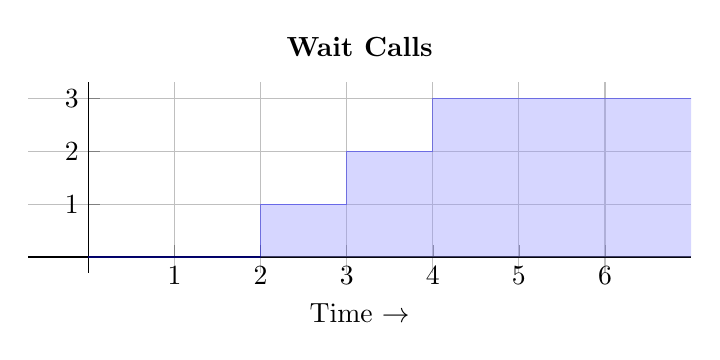
\begin{tikzpicture}
   \begin{axis}[ width=10cm, height=4cm, x axis line style={}, grid =
     major , y axis line style={},
     title={\textbf{Wait Calls}}, xmax=7, axis lines*=center,
     ytick={0,1,2,3,4,5,6}, xtick = {0,1,2,3,4,5,6}, xlabel={Time
       $\rightarrow$}, ylabel={}, xlabel near ticks, ylabel near
     ticks] \addplot [color=blue, domain = 0:6, fill = blue!40!white,opacity=0.4]
     coordinates { (0,0) (2,0) (2,1) (3,1) (3,2) (4, 2) (4,3) (6,3) (8,3) (8,0)};
 \end{axis}
\end{tikzpicture}}
\columnbreak \scalebox{0.7}{
 \hspace{0.5cm}
 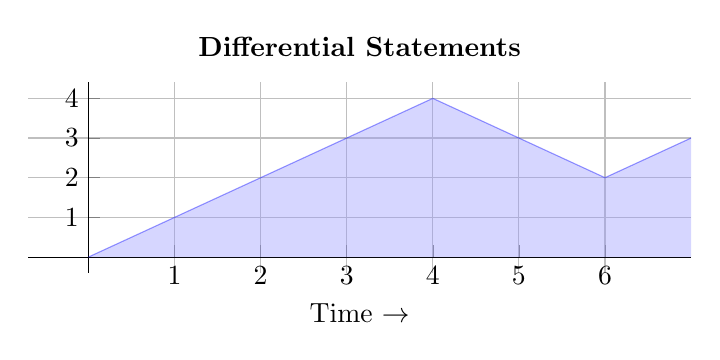
\begin{tikzpicture}
   \begin{axis}[ width=10cm, height=4cm, x axis line style={}, grid =
     major ,y axis line style={},
     title={\textbf{Differential Statements}}, xtick =
     {0,1,2,3,4,5,6} , xmax=7, axis lines*=center,
     ytick={0,1,2,3,4,5,6}, xlabel={Time $\rightarrow$}, ylabel={},
     xlabel near ticks, ylabel near ticks] \addplot [color=blue,
     domain = 0:5, fill = blue!40!white, opacity=0.4 ] coordinates {
     (0,0) (2,2) (4,4) (6,2) (8,4) (8,0)};
 \end{axis}
 \end{tikzpicture}}
\end{multicols}
\hspace{-1cm}

\begin{textblock*}{5cm}(1.1cm,6.2cm)
\scriptsize{$\mathtt{(wait \> 2) \> ; \> x:= x+1 \> ; \> (wait \> 1)}$\ \dots }
\end{textblock*}

\begin{textblock*}{2cm}(7.8cm,6.2cm)
    \scriptsize{$\mathtt{while \> (true) \> \{ }$} \\
    \scriptsize{$\mathtt{\hspace{0.0cm} if \> v \leq 2}$} \\
     \scriptsize{$\hspace{0.8cm} \mathtt{then} \> \hspace{0.1cm}  (\dot{\mathtt{v}} \mathtt{\> = 1 \> for \> 2)}$} \\
    \scriptsize{$\mathtt{\hspace{0.8cm} else \, \,}(\dot{\mathtt{v}}
      \mathtt{\> = -1 \> for \> 2) \>  \> } \}$} 
\end{textblock*}
\end{frame}


\section{Contents of the module}

\begin{frame}{Cyber-Physical \underline{Computation}}

  \begin{minipage}[0.3\textheight]{\textwidth}
  \begin{columns}[c]
  \begin{column}{0.6\textwidth}
    \emph{Genesis}: David Hilbert and its \emph{\alert{Entscheidungsproblem} (\emph{circa} 1928)}
  \end{column}
  \begin{column}{0.2\textwidth}
    \includegraphics[scale=0.15]{Images/Hilbert.jpg}
  \end{column}
  \end{columns}
  \end{minipage}

  \vspace{0.5cm}
  The problem fuelled the appearance of the first two models of computation \dots
  \begin{itemize}
  \item Turing machines (\emph{circa} 1936): state-based computation, part of automata theory
  \item $\lambda$-calculus (\emph{circa} 1936): function-based computation, can be seen as a prototypical
    programming language
  \end{itemize}
\end{frame}

\begin{frame}{Contents of the module pt. I}
  We will study a myriad of models for cyber-physical computation
  \begin{itemize}
  \item timed automata,
  \item a hybrid while-language,
  \item $\lambda$-calculus extended with computational effects (\alert{monads!})
  \end{itemize}

  \pause
  and often make detours through the \alert{mathematical
  foundations} of automata and programming language theory.
\end{frame}

\begin{frame}{Contents of the module pt. II}
  We will also get accquainted with a number of tools
  \begin{itemize}
  \item \alert{Uppaal} -- verification of real-timed systems modelled by (networks of) timed automata
  \item \alert{Lince} -- agile analysis of cyber-physical systems modelled by a hybrid
    while-language
  \item \alert{Haskell} -- a platform to study $\lambda$-calculus
    with effects
  \end{itemize}
\end{frame}

\begin{frame}{How deep will we go into the rabbit hole?}

  \begin{minipage}[1\textheight]{\textwidth}
  \begin{columns}[c]
  \begin{column}{0.8\textwidth}

    Our learning path will intersect theory and practice,
  
    from the very basics to the state-of-the-art ---

    we will face current limitations and see what challenges lie ahead 

  \end{column}
  \begin{column}{0.2\textwidth}
    
    % [...]
    % \includegraphics[scale=1.4]{Images/rabbit.png}
  \end{column}
  \end{columns}
  \end{minipage}

\end{frame}

\section{Logistics}

\begin{frame}{Useful information}
  Relevant class material and announcements will be posted on the website periodically

  \url{https://lmf.di.uminho.pt/CyPhyComp2223}


  E-mail:
    \begin{itemize}
      \item \href{mailto:nevrenato@di.uminho.pt}{nevrenato@di.uminho.pt}
      \item \href{mailto:pro@isep.ipp.pt}{pro@isep.ipp.pt} 
    \end{itemize}
           

  Office hours: wednesday afternoon (please send an email the day before if you wish to meet)
\end{frame}

\begin{frame}{Assessment}
  Assessment will consist of
  \begin{itemize}
  \item 30\% -- an individual test at the end;
  \item 40\% -- a group assignment involving the use of the Uppaal model checker and of Haskell; and %on modelling and analysis of real-timed systems via \texttt{Uppaal} (40\%)
  \item $15\%+15\%$ -- two individual sets of exercises to do at home.
  \end{itemize}
\end{frame}

\end{document}
